% Figure 6 — Counter (Mess) Staff Activities (dark-header box, like the reference)
\documentclass[border=12pt]{standalone}
\usepackage{tikz}
\usepackage[table]{xcolor}
\usetikzlibrary{fit, positioning}
\begin{document}
\small
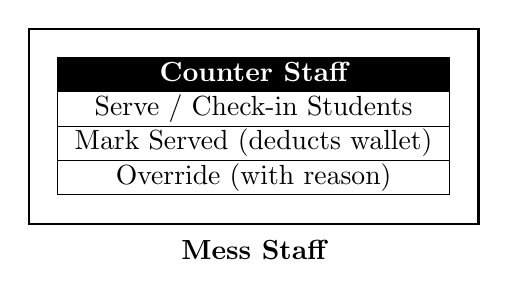
\begin{tikzpicture}
  % Outer frame label "Counter Staff" with its single activity
  \node[inner sep=0pt] (staff) {%
    \begin{tabular}{|c|}
      \hline \rowcolor{black}\color{white}\bfseries Counter Staff \\ \hline
      Serve / Check-in Students \\ \hline
      Mark Served (deducts wallet) \\ \hline
      Override (with reason) \\ \hline
    \end{tabular}};
  \node[draw=black, thick, fit=(staff), inner sep=10pt] (frame) {};
  \node[font=\bfseries, below=2pt of frame] {Mess Staff};
\end{tikzpicture}
\end{document}
